\chapter{Создание таблиц и обеспечение целостности данных}
\section{Создание и изменение таблиц}

\subsection{Создание таблицы}
В T-SQL можно создать таблицу двумя способами: 
\begin{itemize}
	\item с помощью инструкции CREATE TABLE, где явно определяются компоненты таблицы; 
	\item с помощью инструкции SELECT INTO, которая автоматически создает таблицу,
	используя выходные данные запроса для основного определения таблицы. 
\end{itemize}

\begin{figure}[h!]
	\begin{center}
		
\includegraphics[width=0.9\textwidth]{img/advice11.png}
	\end{center}
	\captionsetup{justification=centering}
\end{figure}

\subsection{Определение схемы базы данных}
Каждая таблица принадлежит к группировке объектов внутри базы данных,
которую называют схемой базы данных. Схема базы данных — это поименованный контейнер (пространство имен), который можно использовать для
того, чтобы группировать таблицы и другие объекты баз данных.

\begin{figure}[h!]
	\begin{center}
		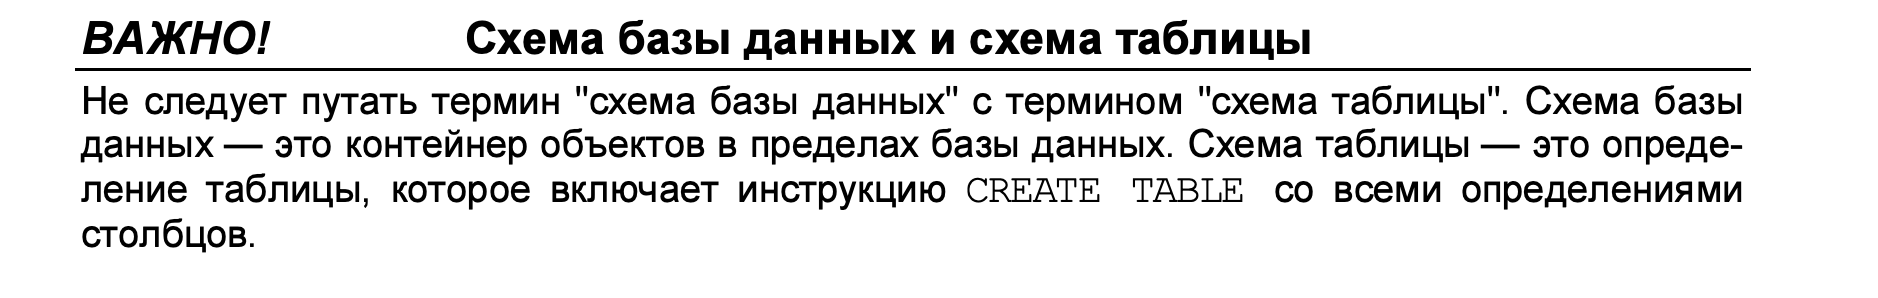
\includegraphics[width=0.9\textwidth]{img/advice12.png}
	\end{center}
	\captionsetup{justification=centering}
\end{figure}

Следующие четыре встроенных схемы баз данных не могут быть удалены: 
\begin{itemize}
	\item схема базы данных dbo — это стандартная (по умолчанию) схема базы данных
	для новых объектов, созданных пользователями, имеющими роли db\_owner или
	db\_ddl\_admin; 
	\item схема guest используется для объектов, которые должны быть доступны пользователю guest. Эта схема используется редко; 
	\item схема INFORMATION\_SCHEMA используется представлениями Information Schema,
	которая предоставляет доступ к метаданным по стандарту ANSI; 
	\item схема базы данных sys зарезервирована SQL Server для системных объектов,
	таких как системные таблицы и представления. 
\end{itemize}

\begin{figure}[h!]
	\begin{center}
		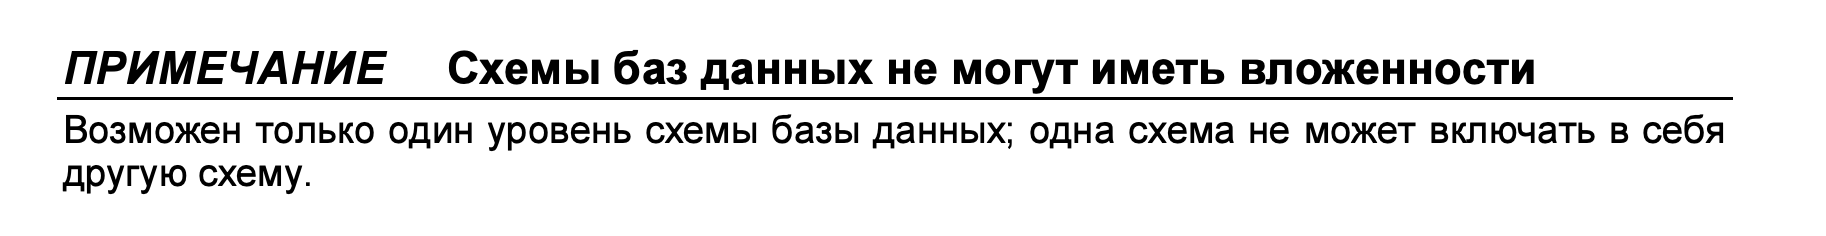
\includegraphics[width=0.9\textwidth]{img/scheme.png}
	\end{center}
	\captionsetup{justification=centering}
\end{figure}

\begin{lstlisting}[label=lst:funcReturn, language=sql]
	CREATE SCHEMA Production AUTHORIZATION dbo;
\end{lstlisting}

Именем схемы Production фактически владеет пользователь с именем dbo, а не схема базы данных dbo. Это позволяет одному пользователю (например, dbo) владеть
несколькими разными схемами базы данных. 


\begin{figure}[h!]
	\begin{center}
		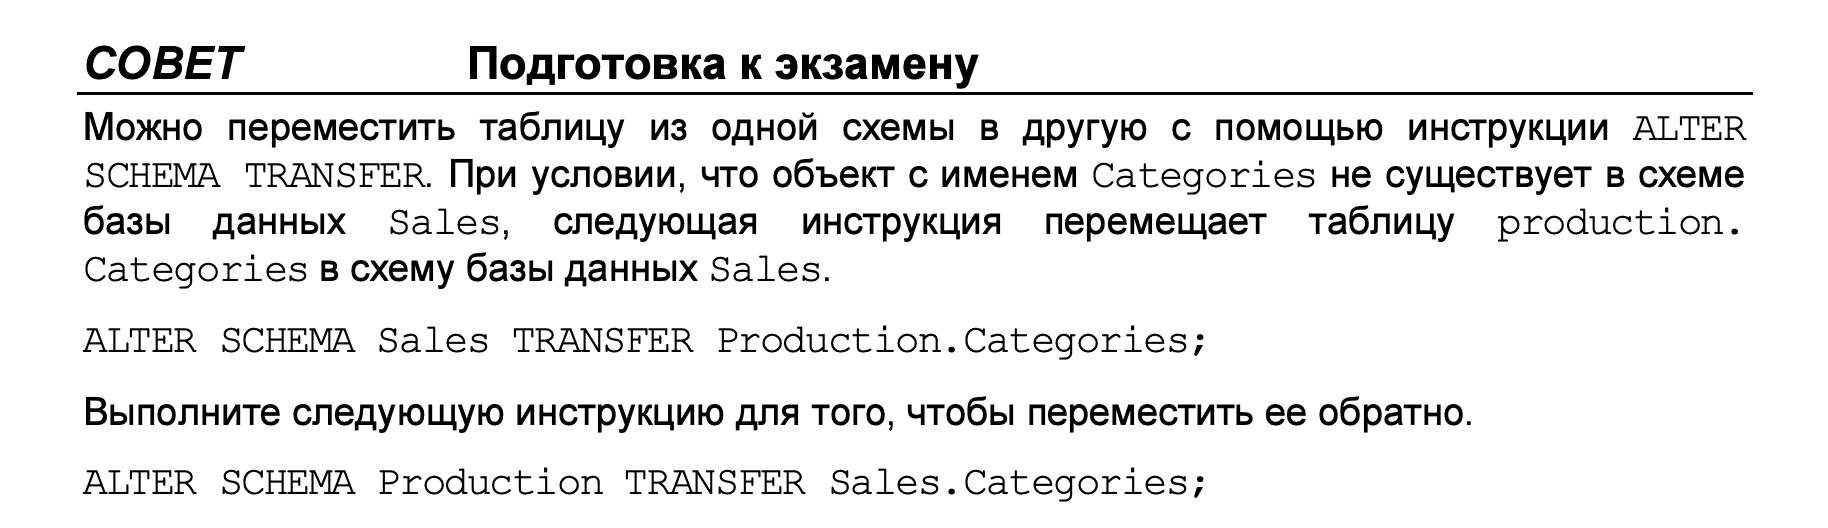
\includegraphics[width=0.9\textwidth]{img/advice13.png}
	\end{center}
	\captionsetup{justification=centering}
\end{figure}

Можно создать таблицу следующим образом: 

\begin{lstlisting}[label=lst:funcReturn, language=sql]
	CREATE TABLE Production.[Yesterday's News] 
\end{lstlisting}

Или это можно записать таким образом: 

\begin{lstlisting}[label=lst:funcReturn, language=sql]
	CREATE TABLE Production."Tomorrow's Schedule" 
\end{lstlisting}

\begin{figure}[h!]
	\begin{center}
		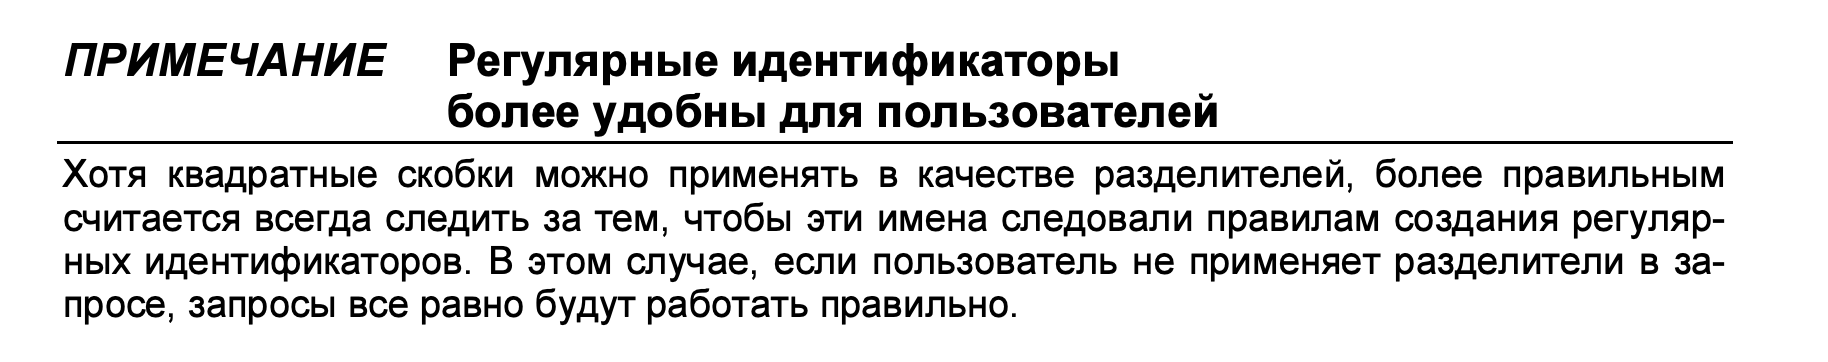
\includegraphics[width=0.9\textwidth]{img/advice14.png}
	\end{center}
	\captionsetup{justification=centering}
\end{figure}


\begin{itemize}
	\item Типы данных DATE, TIME и DATETIME2 могут хранить данные более эффективно и с
	большей точностью, чем типы DATETIME и SMALLDATETIME. 
	\item Используйте типы данных VARCHAR(MAX), NVARCHAR(MAX) и VARBINARY(MAX) вместо
	устаревших типов данных TEXT, NTEXT и IMAGE. 
	\item Используйте тип данных ROWVERSION вместо устаревшего типа TIMESTAMP. 
	\item Типы DECIMAL и NUMERIC — это один и тот же тип данных, но обычно люди предпочитают DECIMAL, поскольку это имя несколько более описательно. Используйте
	типы данных DECIMAL и NUMERIC вместо FLOAT или REAL, кроме случаев, когда вам
	действительно нужна точность с плавающей запятой и известны возможные
	проблемы с округлением. 
\end{itemize}


\begin{lstlisting}[label=lst:funcReturn, language=sql]
	CREATE TABLE Production.Categories(
		categoryid INT IDENTITY(1,1) NOT NULL,
		categoryname NVARCHAR(15) NOT NULL,
		description NVARCHAR(200) NOT NULL DEFAULT ('')
	   ) ON [PRIMARY];
	   GO 
\end{lstlisting}


\subsection{Свойство идентификатора и порядковые номера}
В языке T-SQL свойство идентификатора (identity) может быть назначено столбцу
для того, чтобы автоматически генерировать последовательность чисел. Его можно
применять только к одному столбцу в таблице, и для генерируемой последовательности номеров нужно указать начальное число (seed) и приращение (increment).

\begin{lstlisting}[label=lst:funcReturn, language=sql]
	CREATE TABLE Production.Categories(categoryid INT IDENTITY(1,1) NOT NULL, ... )
\end{lstlisting}

\subsection{Сжатие таблиц}

Существуют два уровня сжатия данных: 

\begin{itemize}
	\item ROW — при сжатии на уровне строк SQL Server применяет более компактный
	формат хранения к каждой строке в таблице; 
	\item PAGE — сжатие на уровне страниц включает в себя сжатие на уровне строк плюс
	дополнительные алгоритмы сжатия, которые могут выполняться на уровне страницы.
\end{itemize}

Следующая команда добавляет сжатие на уровне строк для таблицы
Production.OrderDetails как часть инструкции CREATE TABLE. 

\begin{lstlisting}[label=lst:funcReturn, language=sql]
	CREATE TABLE Sales.OrderDetails
( orderid INT NOT NULL,
 ... )
WITH (DATA_COMPRESSION = ROW);

\end{lstlisting}

\begin{lstlisting}[label=lst:funcReturn, language=sql]
	ALTER TABLE Sales.OrderDetails
	REBUILD WITH (DATA_COMPRESSION = PAGE);
\end{lstlisting}

\begin{figure}[h!]
	\begin{center}
		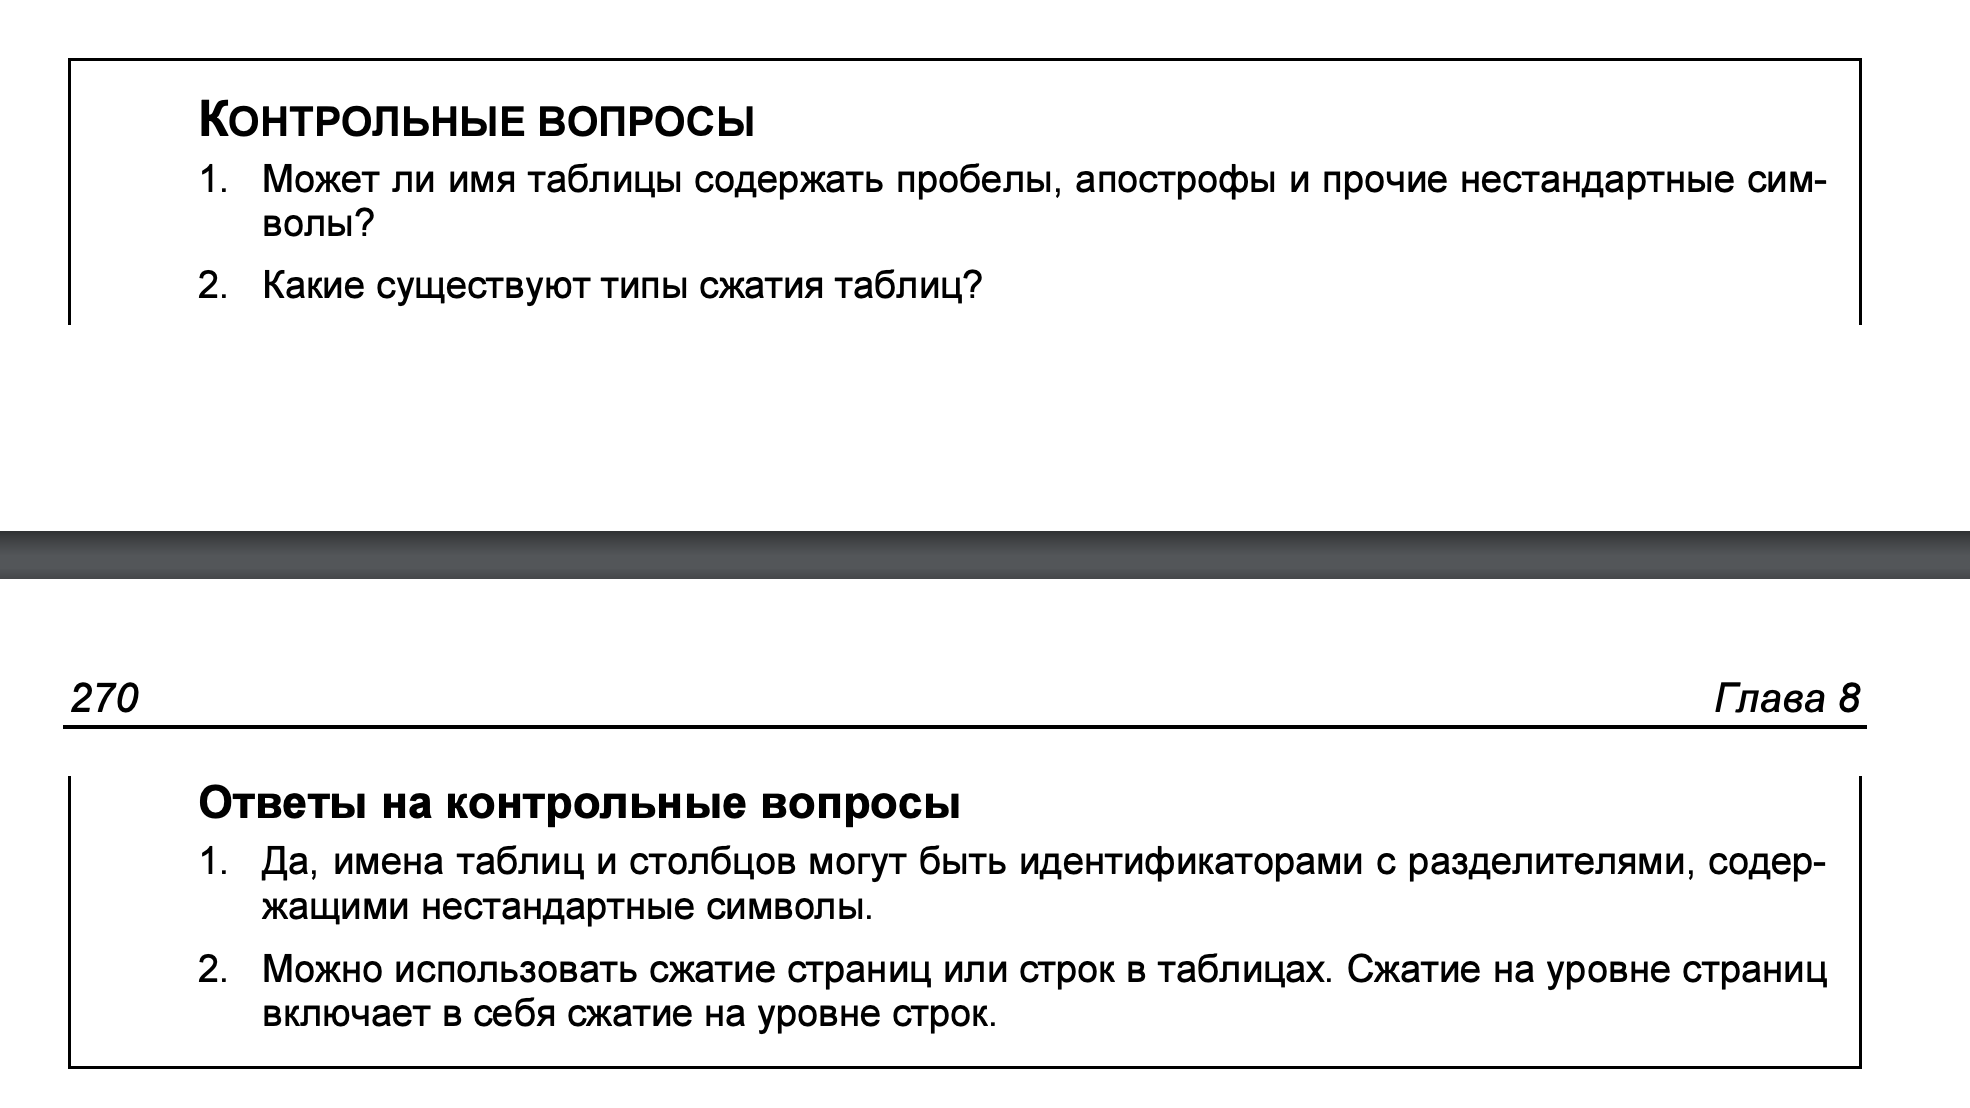
\includegraphics[width=0.9\textwidth]{img/control17.png}
	\end{center}
	\captionsetup{justification=centering}
\end{figure}


\subsection{Изменение таблицы}

Нельзя использовать команду ALTER TABLE для: 
\begin{itemize}
	\item изменения имени столбца; 
	\item добавления свойства идентификатора; 
	\item удаления свойства идентификатора. 
\end{itemize}

\subsection*{Резюме занятия}
\begin{itemize}
	\item При создании таблицы задается схема таблицы как пространство имен или контейнер для таблицы. 
	\item Следует соблюдать аккуратность при присвоении имен таблицам и столбцам и
	делать их описательными. 
	\item Выбирайте наиболее эффективные и точные типы данных для столбцов. 
	\item  Выбирайте подходящие свойства для столбцов, такие как свойство столбца
	IDENTITY, и возможность разрешения в столбце значений NULL. 
	\item Можно задать возможность сжатия таблицы при ее создании. 
	\item Можно использовать команду ALTER TABLE для изменения большинства свойств
	столбцов уже после создания таблицы. 
\end{itemize}

\subsection*{Закрепление материала}

\begin{figure}[h!]
	\begin{center}
		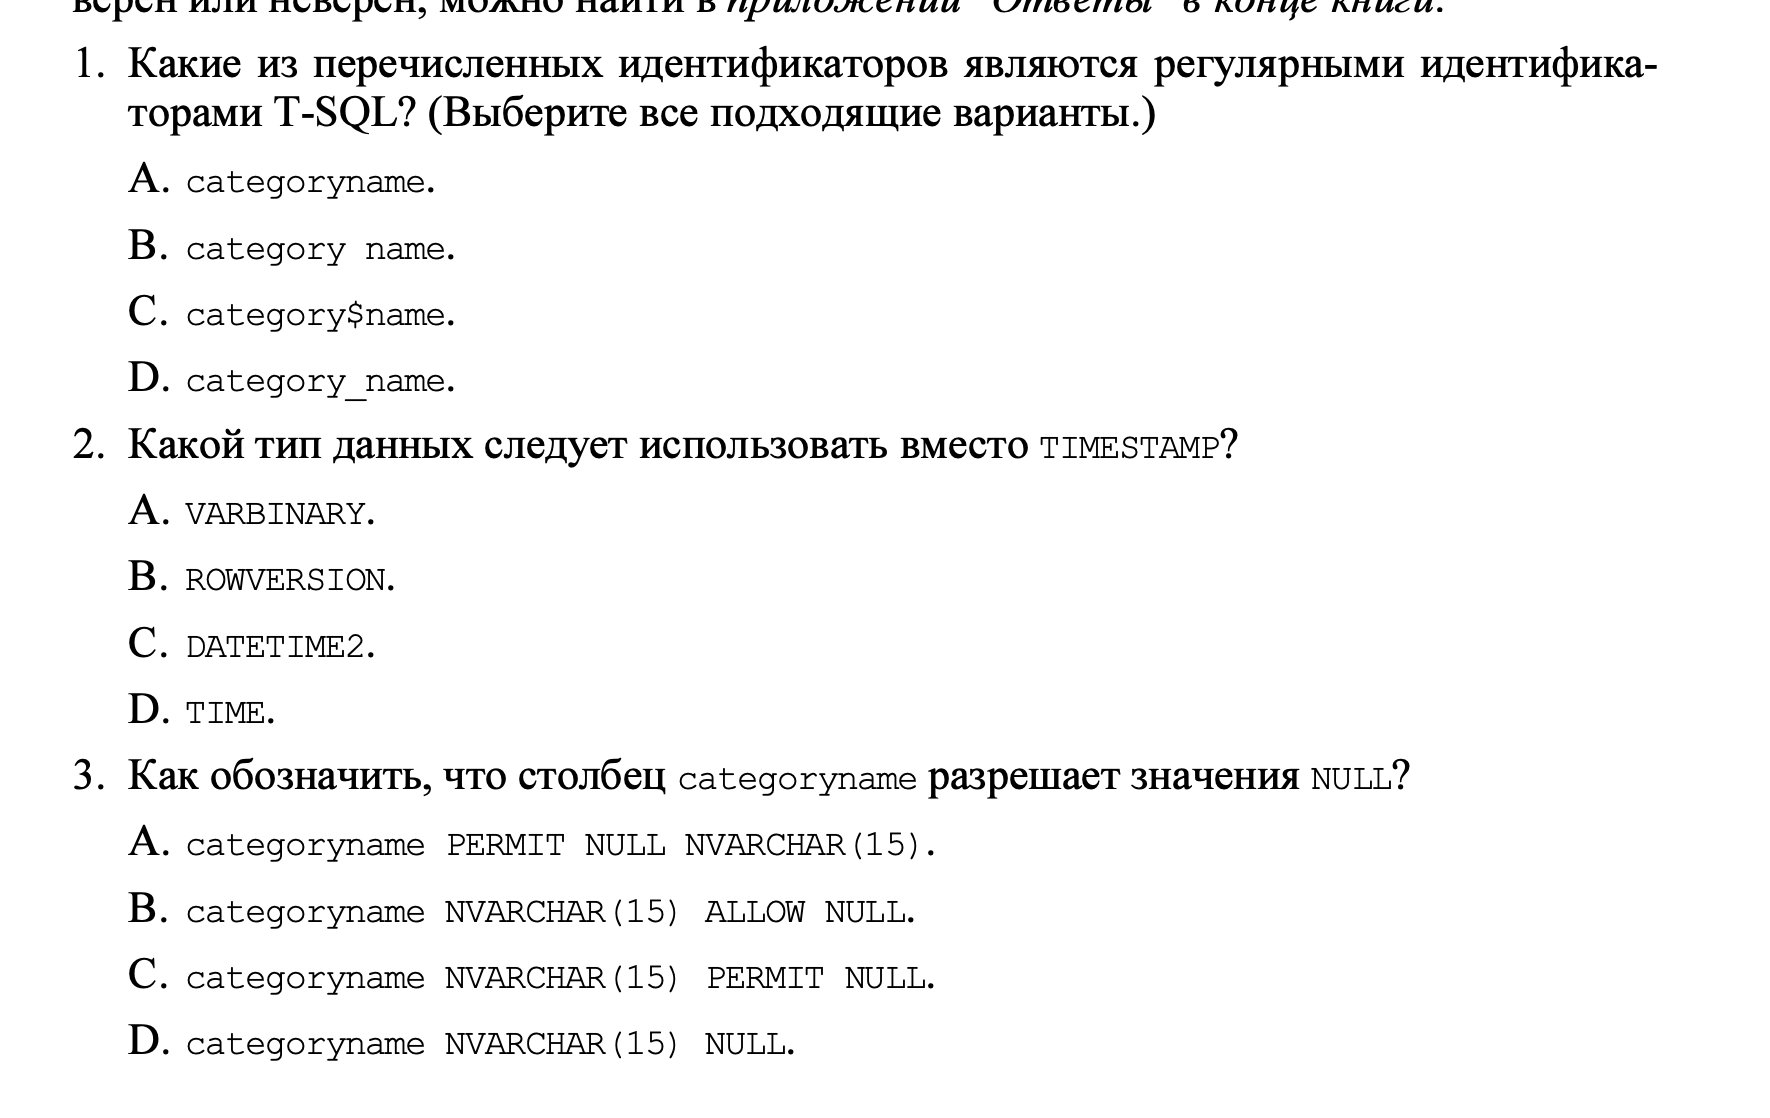
\includegraphics[width=0.9\textwidth]{img/zakrep15.png}
	\end{center}
	\captionsetup{justification=centering}
\end{figure}
\newpage

\subsection*{Ответы}

\begin{figure}[h!]
	\begin{center}
		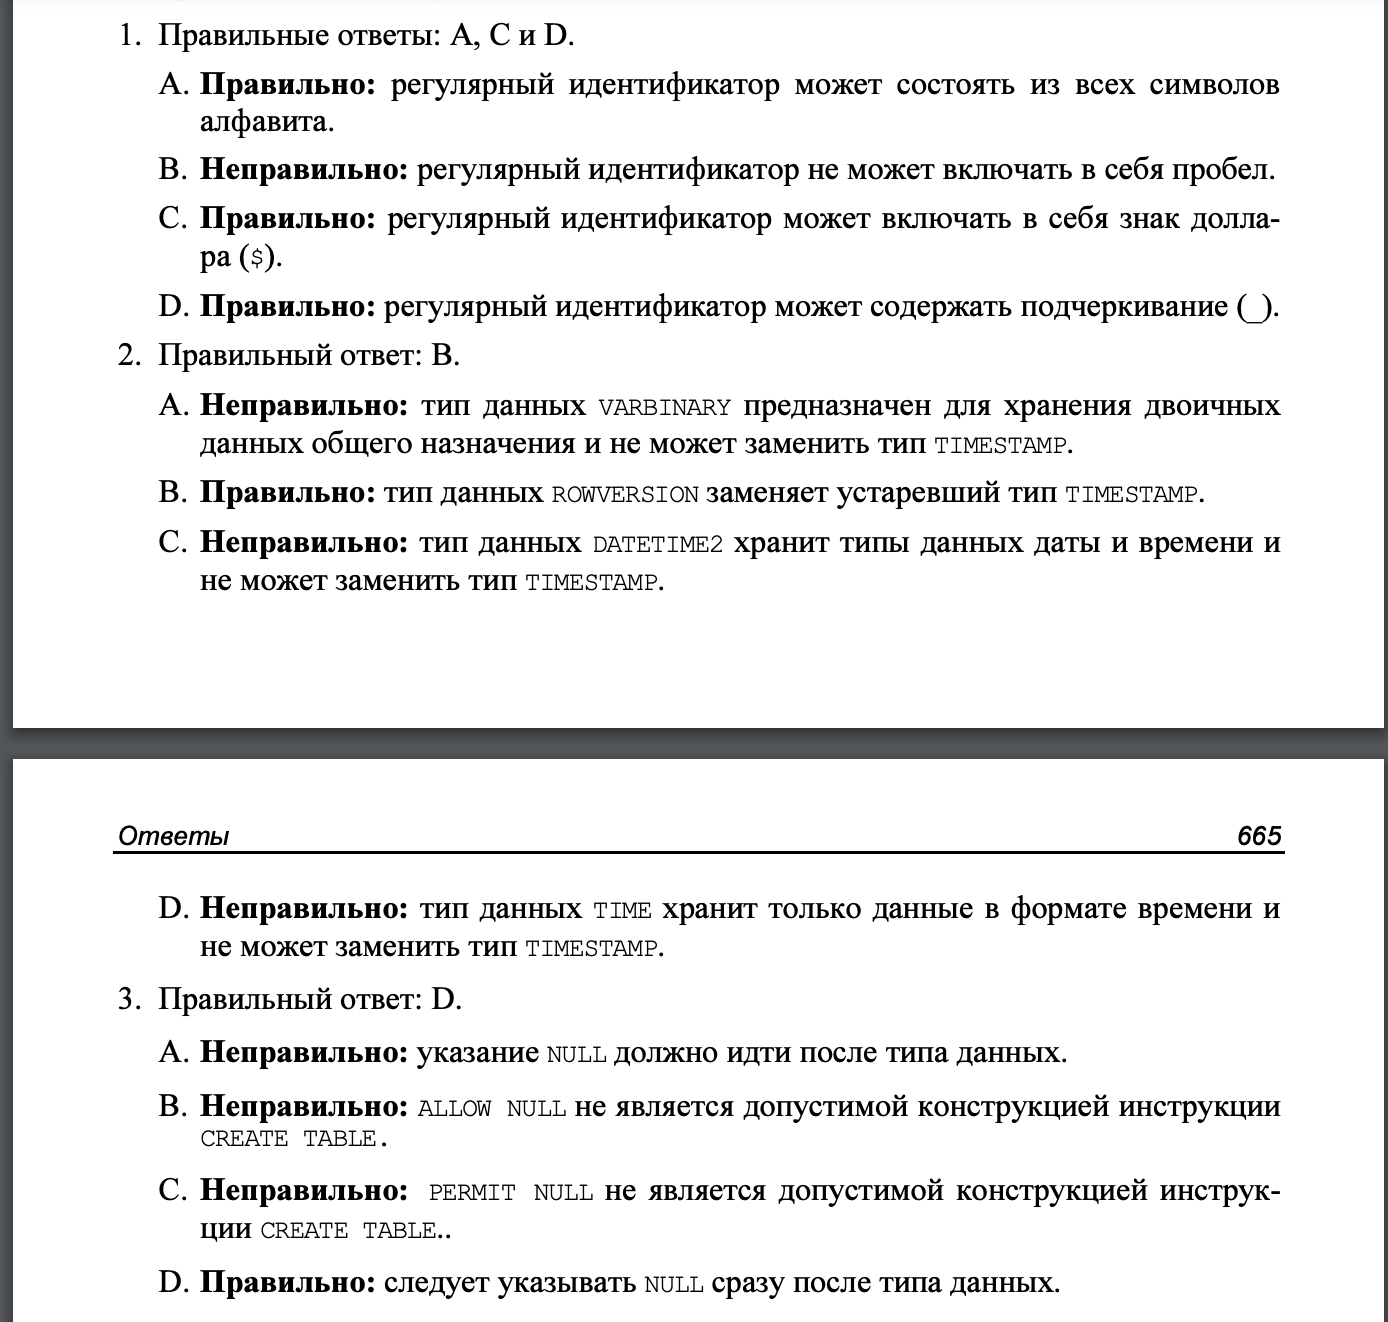
\includegraphics[width=0.9\textwidth]{img/ans16.png}
	\end{center}
	\captionsetup{justification=centering}
\end{figure}
\clearpage


\section{Обеспечение целостности данных}



\subsection{Использование ограничений}


\begin{figure}[h!]
	\begin{center}
		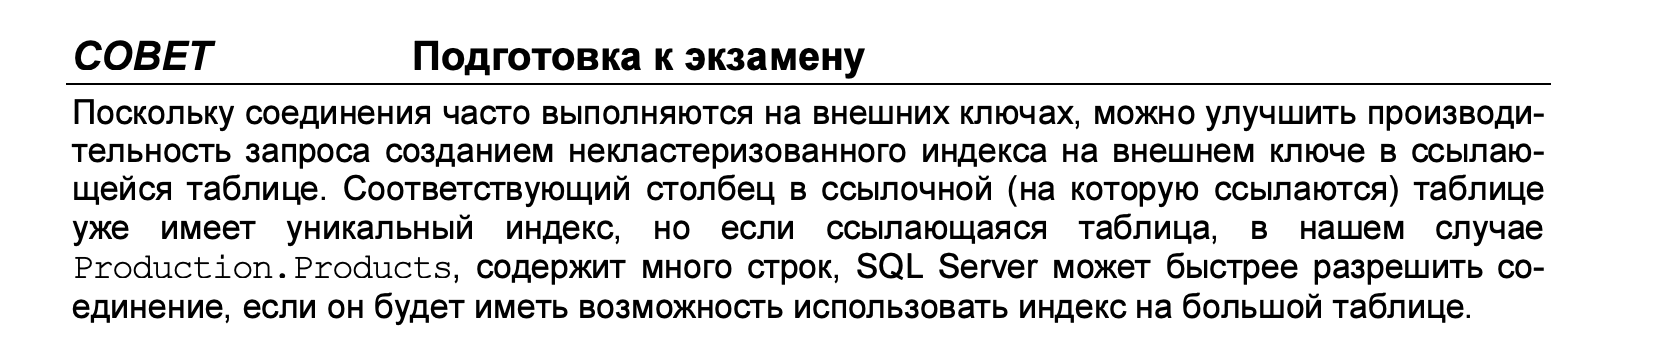
\includegraphics[width=0.9\textwidth]{img/advice15.png}
	\end{center}
	\captionsetup{justification=centering}
\end{figure}

\begin{lstlisting}[label=lst:funcReturn, language=sql]
	CREATE TABLE Production.Products
	( productid INT NOT NULL IDENTITY,
	 productname NVARCHAR(40) NOT NULL,
	 supplierid INT NOT NULL,
	 categoryid INT NOT NULL,
	 unitprice MONEY NOT NULL
	 CONSTRAINT DFT_Products_unitprice DEFAULT(0),
	 discontinued BIT NOT NULL
	 CONSTRAINT DFT_Products_discontinued DEFAULT(0),
	 ... );  
\end{lstlisting}	



		
\subsection*{Резюме занятия}
\begin{itemize}
	\item Для поддержки целостности данных в таблицах базы данных можно объявить
	ограничения, которые сохраняются в базе данных. 
	\item Ограничения обеспечивают подчинение данных, введенных в таблицы, более
	сложным правилам, чем определенные для типов данных и допустимости значений NULL. 
	\item Ограничения таблиц включают в себя ограничения первичного ключа и ограничения уникальности, которые обеспечиваются в SQL Server с помощью уникального индекса. Они также включают ограничения внешнего ключа, гарантирующие, что только данные, правильность которых проверена в другой таблице
	уточненных запросов (lookup table), разрешены в исходной таблице. Также
	к ним относятся проверочные ограничения и ограничения по умолчанию, которые применяются к столбцам. 
\end{itemize}


\subsection*{Закрепление материала}

\begin{figure}[h!]
	\begin{center}
		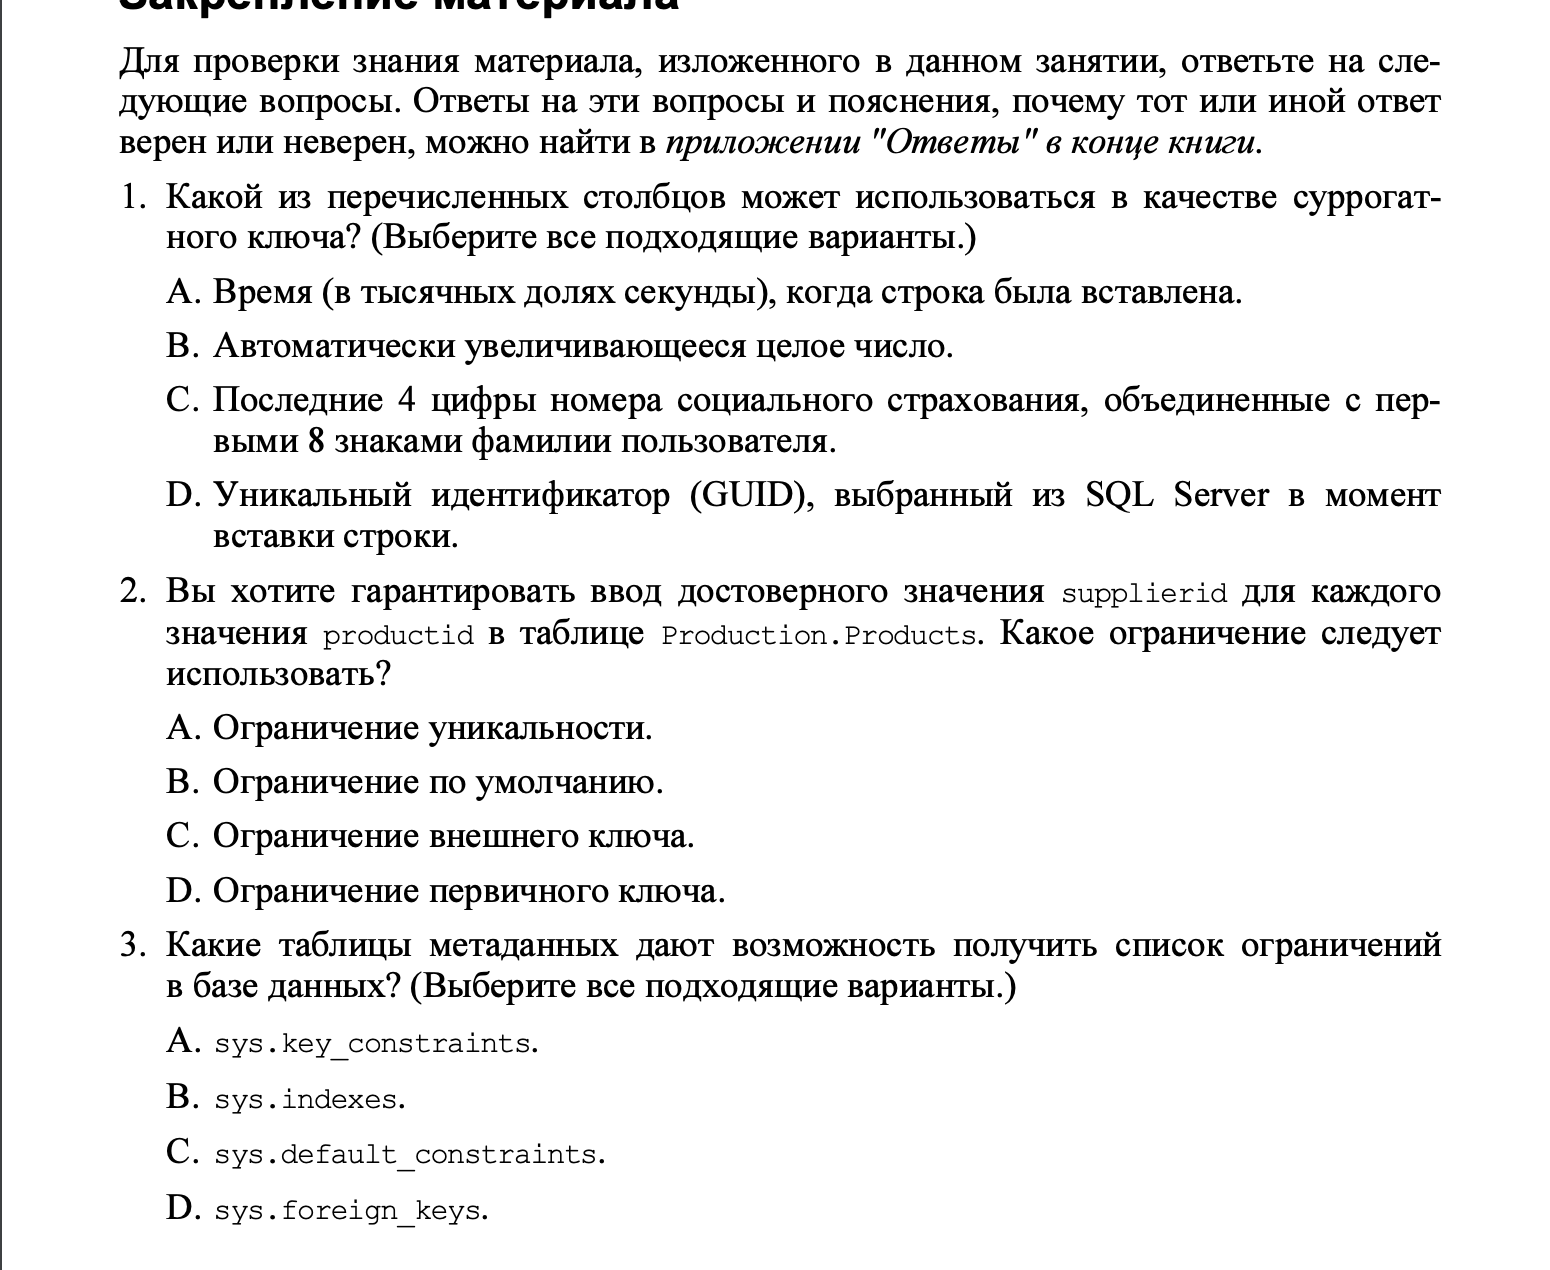
\includegraphics[width=0.9\textwidth]{img/zakrep16.png}
	\end{center}
	\captionsetup{justification=centering}
\end{figure}
\clearpage

\subsection*{Ответы}

\begin{figure}[h!]
	\begin{center}
		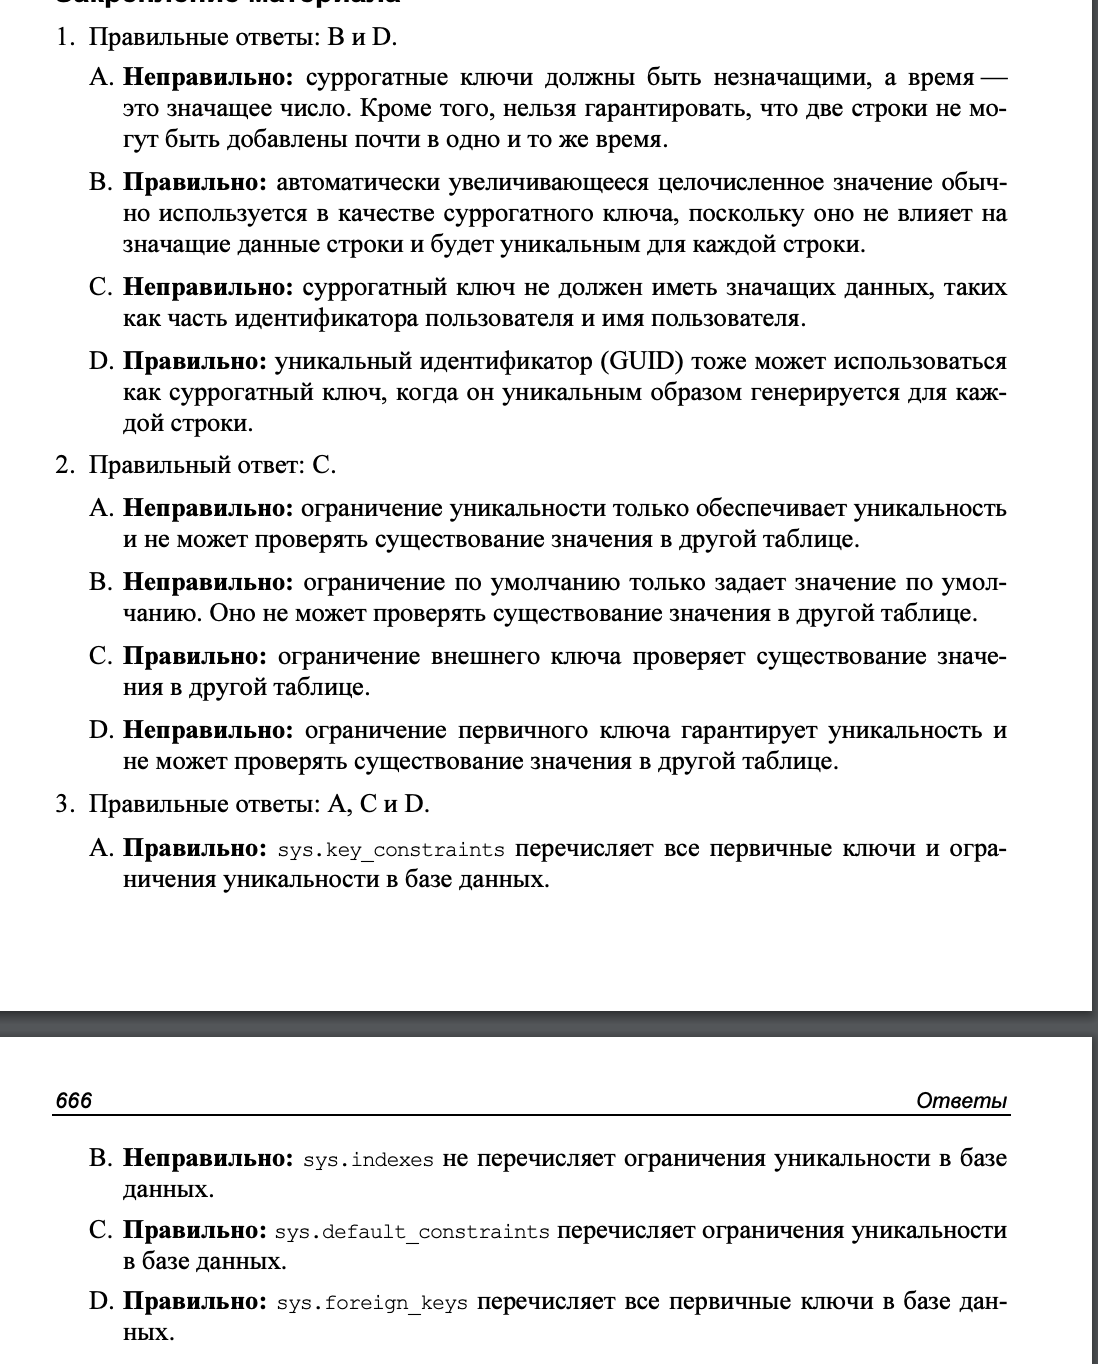
\includegraphics[width=0.9\textwidth]{img/ans17.png}
	\end{center}
	\captionsetup{justification=centering}
\end{figure}

\newpage
\subsection*{Упражнения}

\begin{figure}[h!]
	\begin{center}
		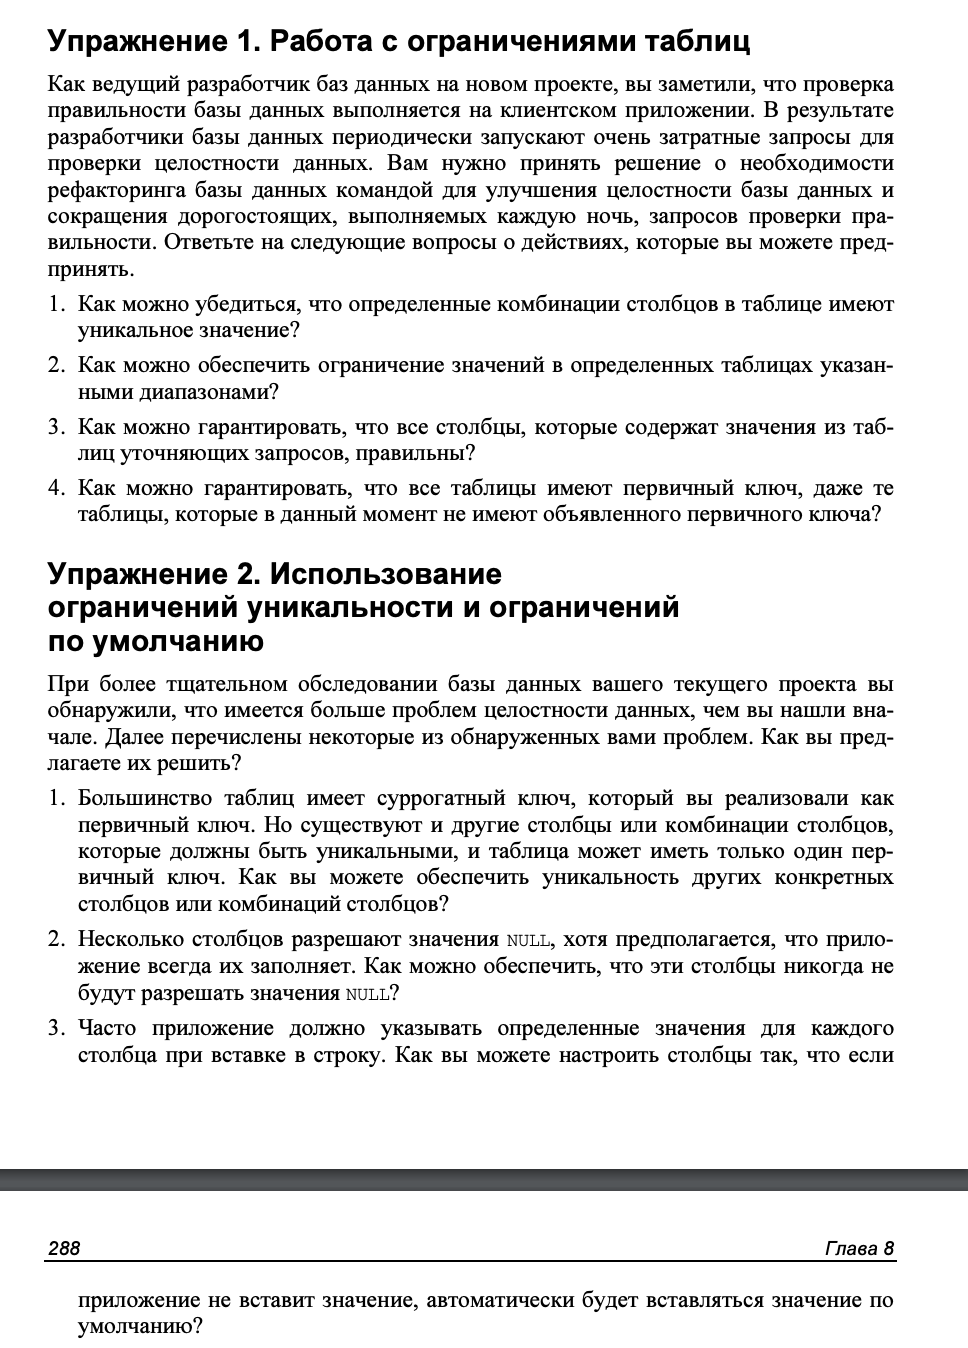
\includegraphics[width=0.9\textwidth]{img/ex14.png}
	\end{center}
	\captionsetup{justification=centering}
\end{figure}

\subsection*{Ответы}

\begin{figure}[h!]
	\begin{center}
		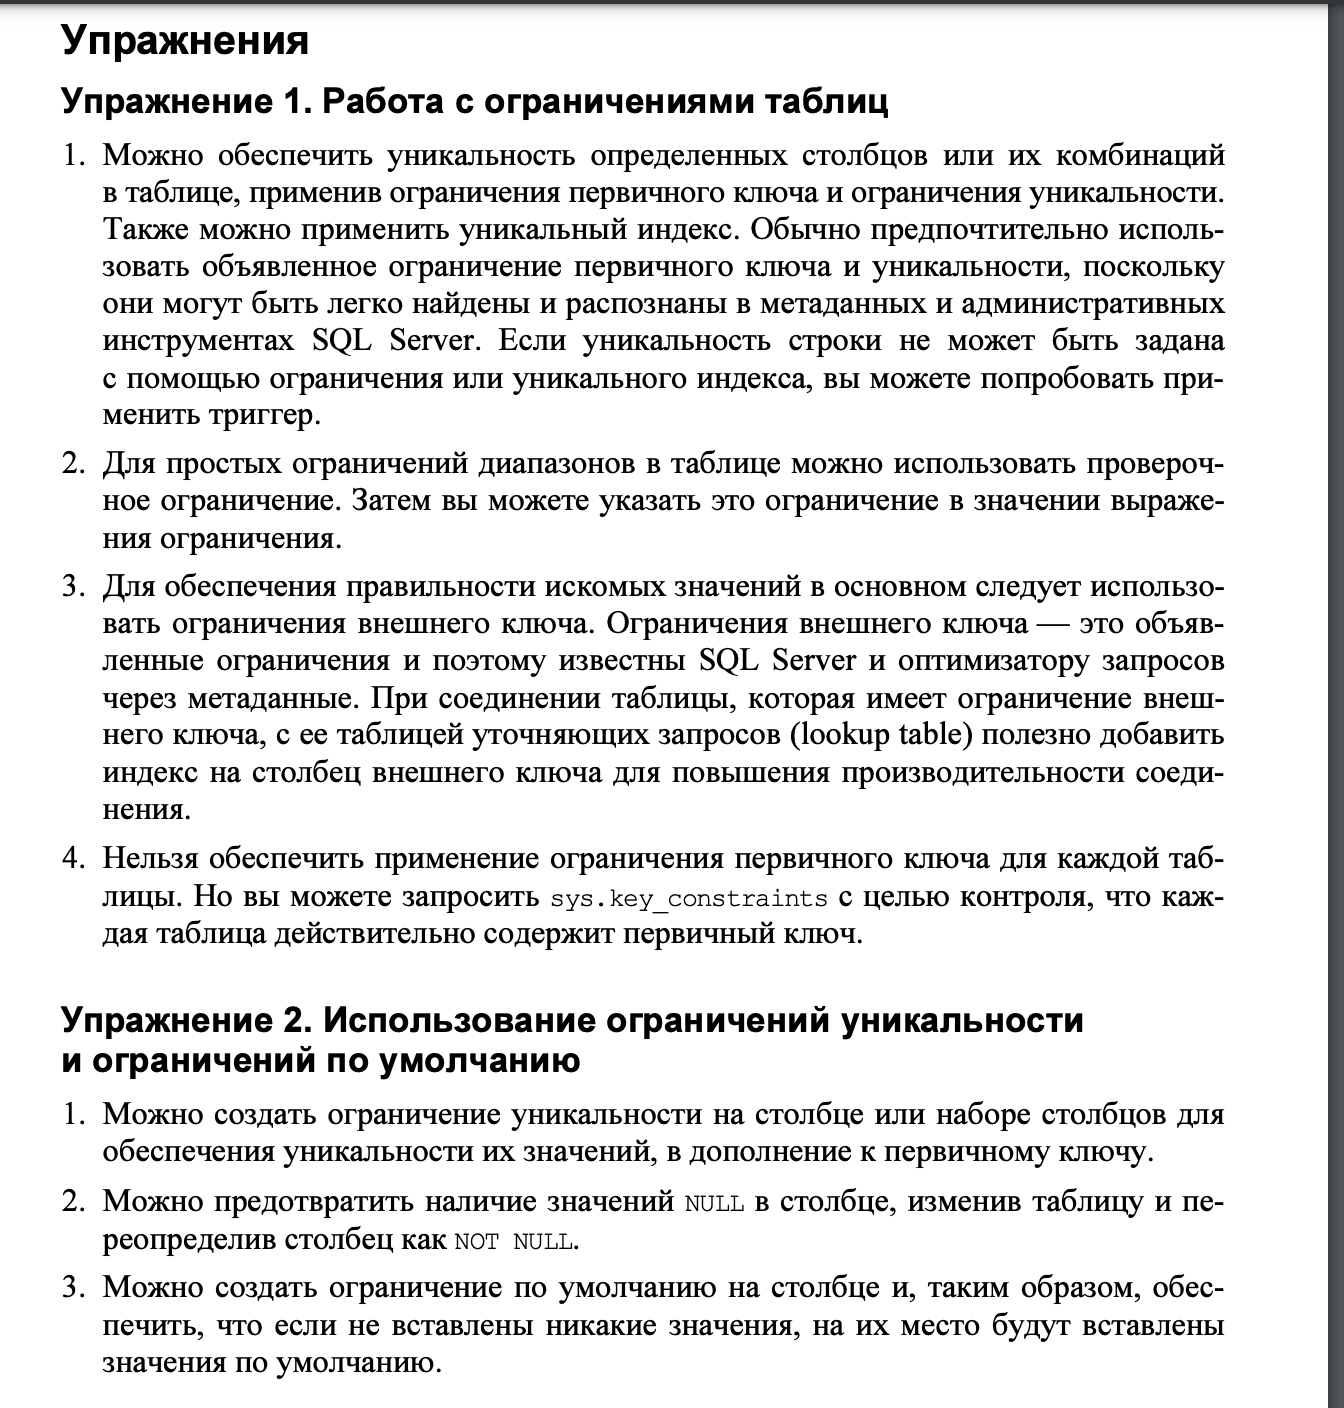
\includegraphics[width=0.9\textwidth]{img/ans18.png}
	\end{center}
	\captionsetup{justification=centering}
\end{figure}





